\documentclass[a4paper]{article}

\usepackage[T1]{fontenc}
\usepackage[utf8]{inputenc}
\usepackage{graphicx}
\usepackage{color}
\usepackage[intlimits]{amsmath}
\usepackage{amsfonts}
\usepackage{listings}
\usepackage{float}
\usepackage{setspace}
\usepackage[english]{babel}
\usepackage{fancyhdr}
\usepackage{booktabs}
\usepackage{multirow}
\usepackage{lastpage}
\usepackage[arrowmos]{circuitikz}
\usepackage[nottoc]{tocbibind}
\usepackage{url}
\usepackage[ugly]{units}
\usepackage[left=1.5cm,top=2cm,right=1.5cm,bottom=2.5cm]{geometry}
\usepackage[pdftex]{hyperref}
\usetikzlibrary{patterns,decorations.pathreplacing,automata,positioning,shapes,arrows}
\usepackage[T1]{fontenc}
%\usepackage{libertine}
\renewcommand*\oldstylenums[1]{{\fontfamily{fxlj}\selectfont #1}}
\setcounter{secnumdepth}{0}

\DeclareMathOperator{\ld}{ld}

\onehalfspacing
\setlength{\parindent}{0pt}

%\widowpenalty=1000
%\clubpenalty=1000

\tocsection

\author{Iffat Brekhna}

\setcounter{tocdepth}{4}
\setcounter{secnumdepth}{4}
\begin{document}
	\pdfinfo
	{/Creator (Iffat Brekhna)
	 /Producer (pdflatex)
	 /Author (Iffat Brekhna)
	}

\pagestyle{fancy}
\fancyhead{}
\fancyfoot{}
\renewcommand{\headrulewidth}{0pt}
\begin{center}

\begin{tabular*}{\textwidth}{@{\extracolsep{\fill}}lr}
	\textbf{Lehrstuhl für Integrierte Systeme} & \textbf{Technische Universität München} \\
	\includegraphics[height=1cm]{lis_logo.png} &
	
\begin{tikzpicture}[x=0.2cm,y=0.2cm]
		\definecolor{tum}{rgb}{0,0.396078,0.741176}
		\fill[fill=tum]
		      (0,5)
		   -- (0,4)
		   -- (1,4)
		   -- (1,0)
		   -- (2,0)
		   -- (2,4)
		   -- (3,4)
		   -- (3,0)
		   -- (6,0)
		   -- (6,4)
		   -- (7,4)
		   -- (7,0)
		   -- (8,0)
		   -- (8,4)
		   -- (9,4)
		   -- (9,0)
		   -- (10,0)
		   -- (10,5)
		   -- (5,5)
		   -- (5,1)
		   -- (4,1)
		   -- (4,5)
		   -- cycle;
	\end{tikzpicture}
\end{tabular*}

\vfill

\huge{Project Lab IC-Design}

\huge{Projektpraktikum IC-Entwurf}

\large{Summer Semester 2017}

\vfill

%\huge\textbf{Group X}
\huge\textbf{Iffat Brekhna}
\\
%\large\textit{Iffat Brekhna \\ Matriculation Number: 03670102}
\large\textit{Matriculation Number: 03670102}

\end{center}

\newpage

\renewcommand{\headrulewidth}{0pt}
\setlength{\parskip}{6pt}
\renewcommand{\headrulewidth}{.4pt}
%\fancyhead[r]{Iffat Brekhna, group X}
\fancyhead[r]{Iffat Brekhna}
\fancyhead[c]{Projektpraktikum IC-Entwurf}
\fancyhead[l]{Technische Universität München}
\fancyfoot[c]{Page \thepage\ of \pageref{LastPage}}

\tableofcontents
\newpage

\section{Display Module}

\subsection{Introduction}

The display module receives input lines from all other modules in BCD format. It has a display driver which is responsible for initializing the LCD using the control signals. The display module decides which data should be displayed at a certain time, in other words, it forward the data of the mode the clock module is in. The current mode input is received from the global Finite State Machine (FSM) as a 3 bit input. Figure~\ref{fig:FUNC} shows the functional specification of the display module. There was no issue with managing the timing issues in this module because our clock module is running with a system clock (clk) of 10KHz. This makes the time period to be 1000us which is much larger then the minimum timing constraints given in the data sheet of the LCD for the operations that we do. 

\begin{figure}[h!]
  \begin{center}
    \includegraphics[width=0.7\textwidth]{FUNC.png}
    \caption{Functional specification}
    \label{fig:FUNC}
  \end{center}
\end{figure}

\subsection{Implementation}
The register transfer level (RTL) logic of the display driver is shown in Figure~\ref{fig:RTL}. The internal signals are defined below:
\begin{itemize}
	\item $line$ : selects the lines to be saved in the register file
	\item $r\_en$ :  enable for register in write cycle
	\item $lines\_done$ : signal to notify the LCD FSM when all the words of the 2 lines from the register file are written into the DDRAM in the LCD module
	\item $tx\_done$ : signal from the control FSM to notify whenever a single word is written into the DDRAM of the LCD
	\item $addr\_mux$ : address of the word to read from the register file
	\item $data\_out$ : output from the register file i.e data to be displayed in the LCD
	\item $fsm\_data$ : control data from the LCD FSM
	\item $Data$ : The data to be written into the LCD DDRAM
	\item $RS$ : Register select to determine whether it is a instruction entry or a data entry
	\item $R/W$ : It is always tied to 0 because we are always only writing data to the LCD DDRAM 
	\item $E$ : Enable for sampling of data 
\end{itemize}

\begin{figure}[h!]
  \begin{center}
    \includegraphics[width=0.7\textwidth]{RTL1.png}
    \caption{Register Transfer Logic of the display driver}
    \label{fig:RTL}
  \end{center}
\end{figure}
 
\subsubsection{Register File}
The Register File's size is 320 bits so that it can save two lines at a time. The input to this register file is either line 1 concatenated with line 3 or line 2 concatenated with line 4 because in the LCD module the DDRAM address space is divided in a way that line 1 address is followed by line 3 address and line 2 address is followed by line 4 address. So it's easier to write data in the DDRAM in this way rather than writing one line, changing the DDRAM address and then writing another line for all four lines. 

\subsubsection{LCD Display FSM}
Figure~\ref{fig:LCD_FSM} shows the FSM diagram of this block. It is responsible for the initialization phase of the LCD and also the display functionality. The signal `D' defined in this module is the same signal defined as $fsm\_data$ in the RTL logic of the display driver. It was shortened to D due to space issues while drawing the FSM in \LaTeX. Each state is defined below.\\

\begin{itemize}
	\item $S_0$ : It is the first step of LCD initialization in which the function set step is executed. D = 0x38 means setting a 8-bit bus mode with MPU, having a 2-line display mode and a 5x8 dot format display mode set.
	\item $S_1$ : It is the second step of LCD initialization in which the display is turned on. D = 0x0C means that the entire display is turned on, the cursor is off and blink is off.
	\item $S_2$ : It sets the DDRAM address. D=0x80 means the address is set to line 1.
	\item $S_3$ : It writes the data from the register file into the LCD DDRAM. D=X means that it can be any data depending on the input from the outside (other modules). The FSM continues to be in this state unless both the lines (line 1 and 3) are written into the DDRAM i.e it switches to the next state when $lines\_done$ = 1.
	\item $S_4$ : It sets the DDRAM address. D=0xC0 means the address is set to line 2.
	\item $S_5$ : It writes the data from the register file into the LCD DDRAM. D=X means that it can be any data depending on the input from the outside (other modules). The FSM continues to be in this state unless both the lines (line 2 and 4) are written into the DDRAM i.e it switches to the next state when $lines\_done$ = 1.
\end{itemize}

\begin{figure}[h!]
	\begin{center}
		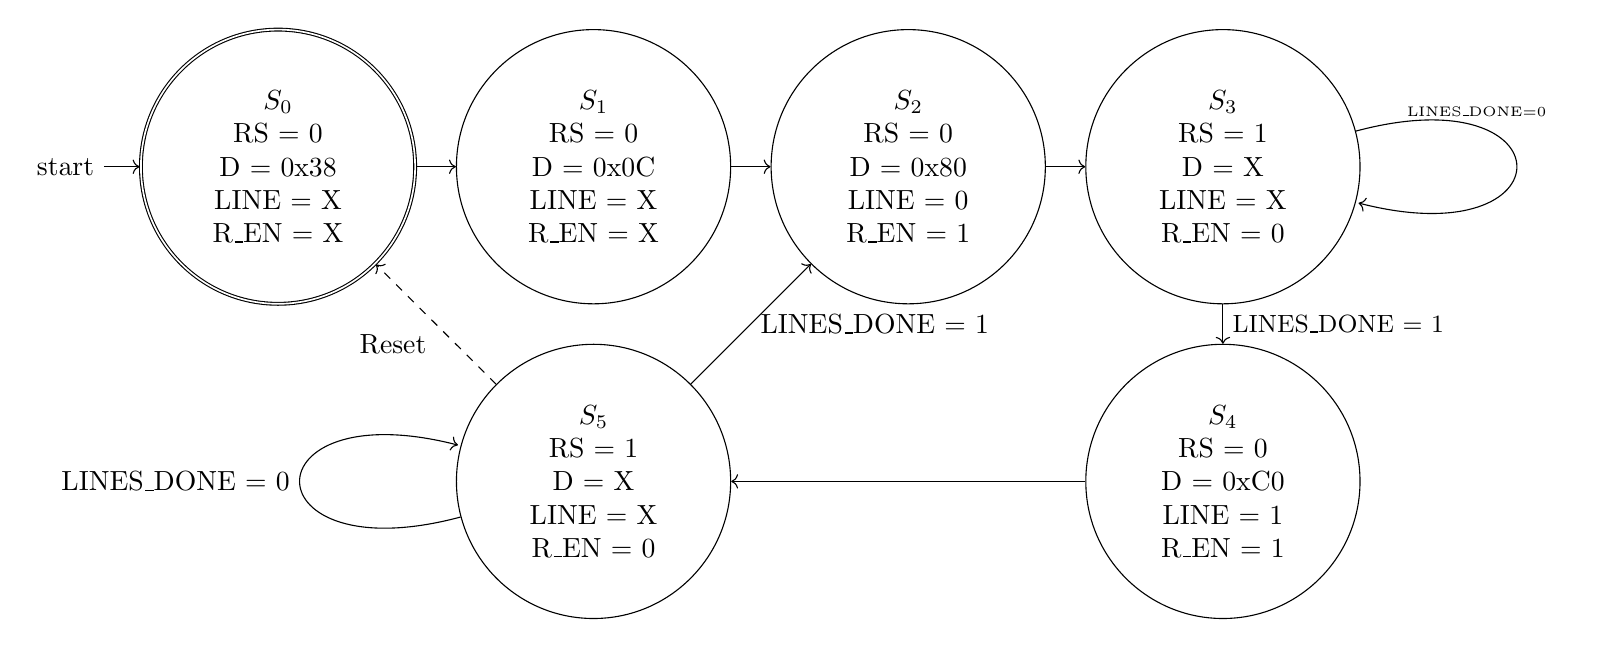
\begin{tikzpicture}[every state/.style={text width=2.5cm,align=center,node distance=0.5cm},auto]
			\node[state,accepting,initial]  (DisplayOn)  { \textbf{$S_0$}\\ RS = 0 \\ D = 0x38 \\ LINE = X \\ R$\_$EN = X };
			\node[state,right=of DisplayOn]  (Function) { \textbf{$S_1$} \\ RS = 0 \\ D = 0x0C \\ LINE = X \\ R$\_$EN = X };
			\node[state,right=of Function] (SetAddr1) { \textbf{$S_2$} \\ RS = 0 \\ D = 0x80 \\ LINE = 0 \\ R$\_$EN = 1 };
			\node[state,right=of SetAddr1] (Write1)   { \textbf{$S_3$} \\ RS = 1 \\ D = X    \\ LINE = X \\ R$\_$EN = 0 };
			\node[state,below=of Write1]   (SetAddr2) { \textbf{$S_4$} \\ RS = 0 \\ D = 0xC0 \\ LINE = 1 \\ R$\_$EN = 1 };
			\node[state,below=of Function] (Write2)   { \textbf{$S_5$} \\ RS = 1 \\ D = X    \\ LINE = X \\ R$\_$EN = 0 };

			\path[->]
						 (DisplayOn)  edge                    (Function)
						 (Function) edge       			  (SetAddr1)
						 (SetAddr1) edge             	     (Write1)
						 (Write1)   edge            		 node {\small{LINES$\_$DONE = 1}}    (SetAddr2) edge[loop right,near start,above] node {\tiny{LINES$\_$DONE=0}} ()
						 (SetAddr2) edge                      (Write2)
						 (Write2) 	 edge[loop left]  node {LINES$\_$DONE = 0}  ()
						 (Write2)  edge   node [right]{LINES$\_$DONE = 1} (SetAddr1);
						
							 
			\path[->, dashed]  (Write2)  edge   node {Reset} (DisplayOn);
		\end{tikzpicture}	
	\end{center}
	\caption{LCD Display FSM. All transitions not labeled occur on CLK$\uparrow$ if $tx\_done$ = 1}
	\label{fig:LCD_FSM}	
\end{figure}

\subsubsection{Control Signals FSM}
Figure~\ref{fig:control_FSM} shows the FSM diagram of this block. It is responsible for generating the control signals which are inputs to the LCD FSM, the counter and it also generates the `E' signal of the LCD. The $tx\_done$ signal represents the transmission of a single block of data (one character) to the LCD DDRAM.


\subsubsection{Counter}
The counter is incremented when $r\_en$ = 0, $tx\_done =1$ and $RS$ = 1. When the count value equals 39 the signal $lines\_done$ = 1 implying that all 40 characters have been written into the DDRAM of the LCD. Also, the $addr\_mux$ signal is calculated by subtracting the count value of the counter from 39 to take care of the order of reading data from the register file.

\begin{figure}[H]
	\begin{center}
		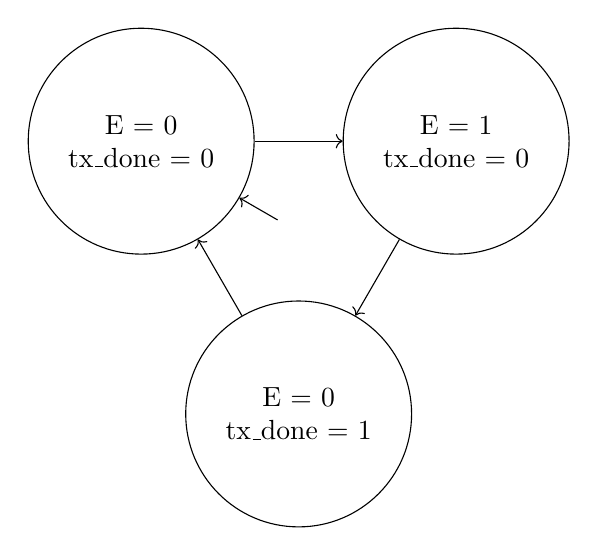
\begin{tikzpicture}[every state/.style={text width=2.5cm,align=center,node distance=.5cm},auto]
			\node[state] (S0) at (0.0,0) {  E = 0 \\ tx$\_$done = 0 };
			\node[state] (S1) at (4.0,0) {  E = 1 \\ tx$\_$done = 0 };
			\node[state] (S2) at (-60:4) {  E = 0 \\ tx$\_$done = 1 };

			\path[->] (S0) edge (S1)
						 (S1) edge (S2)
						 (S2) edge (S0)
						 (S0) ++ (-30:2) edge (S0);
		\end{tikzpicture}
	\end{center}
	\caption{Control Signals FSM. All transitions occur on CLK$\uparrow$}
	\label{fig:control_FSM}
\end{figure}

\section{Changes from the Initial Presentation}
In the initial presentation, I presented some things which while writing the code I realized had to be changed. First of all, the functional specification of the display module as shown in figure~\ref{fig:FUNC} has been changed. In the initial presentation it was proposed that data is received from other modules as $std\_logic\_vectors$. However, this format has been changed to BCD. Also initially, the time display was always forwarded to the display driver regardless of the state the clock module was in but later this logic was also changed as the Time Switch states had to be taken care of. 
\par
Secondly, the register transfer level (RTL) logic of the display driver as shown in figure~\ref{fig:RTL} has been modified. In the previous version there was no mux in front of the register file to read each word. An issue arose while reading from the register file and the order to read in as the display was displaying everything in the wrong order. To solve that issue, a mux was added and the select line of the mux ($addr\_mux$) was set in such a way that it reads the line from left to right i.e in the order the line has to be displayed. 
\par
Thirdly, the $LCD\_DISPLAY\_FSM$ module as shown in figure~\ref{fig:LCD_FSM} also had a logical error. In the initial presentation I proposed turning ON the LCD first and then setting the mode but after several tries of failing to run the LCD I found out that the order was wrong, I was supposed to set the mode first and then turn the LCD ON. So the order of the first two states changed. 

\section{Results}
Figure~\ref{fig:LCD_FSM_SC} shows the simulation results of the LCD FSM module. 
Figure~\ref{fig:CONTROL_FSM_SC} shows the simulation results of the Control FSM module. Figure~\ref{fig:simulation} shows the simulation results of the Display Driver. The LCD is running perfectly fine in real life as well (as demonstrated in the demo).

\begin{figure}[h!]
  \begin{center}
    \includegraphics[width=\textwidth]{LCD_FSM_SC.png}
    \caption{Simulation Results of the LCD FSM Module}
    \label{fig:LCD_FSM_SC}
  \end{center}
\end{figure}

\begin{figure}[h!]
  \begin{center}
    \includegraphics[width=\textwidth]{CONTROL_FSM_SC.png}
    \caption{Simulation Results of the Control FSM Module}
    \label{fig:CONTROL_FSM_SC}
  \end{center}
\end{figure}
 
\begin{figure}[h!]
  \begin{center}
    \includegraphics[width=\textwidth]{simulation.png}
    \caption{Simulation Results of the Display Driver}
    \label{fig:simulation}
  \end{center}
\end{figure}

\end{document}


